\chapter{RESULTADOS}

% ======================================================================
% CAPITULO 5 - RESULTADOS. Secciones de Fase 1 (OE1) y Fase 2 (OE2).
% Reemplaza las lineas 13-71 de cap5-resultados.tex (desde
% \section{Fase 1...} hasta justo antes de \section{Fase 3}).
%
% Figuras requeridas en images/ (copiar desde fase1_khipu/figuras/figs/):
%   fig1_embudo_seleccion.pdf      fig2_calidad_genomica.pdf
%   fig3_arbol_filogenomico.pdf    fig4_matriz_mash.pdf
%   fig5_novedad_taxonomica.pdf    fig6_prevalencia_linajes.pdf
%   fig7_composicion_taxonomica.pdf
% ======================================================================

\section{Fase 1. Control de calidad y selección de genomas (OE1)}

La Fase 1 se ejecutó en el clúster Khipu mediante el controlador
\texttt{run\_fase1.slurm} (trabajo SLURM 49286), sobre los 97 bins genómicos
crudos procedentes de las 22 librerías Illumina que recuperaron material
ensamblable (Tabla~\ref{tab:bins}). El flujo aplicó dos filtros secuenciales e
independientes: primero una discriminación por dominio con Tiara y después una
estimación de calidad genómica con CheckM2. El orden no es intercambiable, ya
que las métricas de completitud y contaminación de CheckM2 se calculan sobre
marcadores procariotas y carecen de sentido en un ensamblaje
mayoritariamente eucariota.

\subsection{Depuración secuencial del conjunto de bins}

El filtrado por dominio descartó 31 de los 97 bins, cuya mayoría se
clasificó como eucariota u organelar. Este resultado era esperable dado el
origen de las muestras: una superficie pétrea expuesta a la intemperie acumula
material fúngico, algal y vegetal que el ensamblaje por muestra no separa del
componente procariota. Casos como \texttt{bin-1-55}, con 34.2 Mb repartidos en
247 contigs, corresponden con claridad a un genoma eucariota parcialmente
reconstruido y no a un genoma bacteriano contaminado.

Los 66 bins restantes pasaron al control de calidad genómica, donde se aplicó el
criterio definido para el OE1: completitud superior al 70\% y contaminación
inferior al 5\%. De ellos, 45 fueron rechazados y 21 seleccionados, lo que
representa una tasa de retención del 21.65\% sobre el total crudo inicial. El
motivo de los rechazos resulta informativo porque distingue dos problemas de
naturaleza distinta:

\begin{itemize}
    \item \textbf{18 bins} incumplieron únicamente el criterio de completitud
    ($\le 70\%$). Se trata de reconstrucciones parciales, atribuibles a baja
    profundidad de secuenciación o a fragmentación del ensamblaje. Los valores
    cubren todo el rango, desde reconstrucciones cercanas al umbral, como
    \texttt{bin-1-50} con 62.29\%, hasta fragmentos residuales sin utilidad
    analítica, como \texttt{bin-1-52} con 6.05\%.
    \item \textbf{20 bins} incumplieron únicamente el criterio de contaminación
    ($\ge 5\text{\%}$), lo que indica quimerismo: contigs de linajes distintos
    coagrupados por MetaBAT2 durante el \textit{binning}. La magnitud es en
    ocasiones considerable, como en \texttt{bin-1-60}, con 24.87\%.
    \item \textbf{7 bins} incumplieron ambos criterios de forma simultánea. El
    caso extremo es \texttt{bin-1-58}, con 0.00\% de completitud y 17.71\% de
    contaminación, un agrupamiento sin correspondencia con ningún genoma real.
\end{itemize}


Esta diferencia es importante para entender qué se perdió en cada caso. Los 18 bins incompletos corresponden a información que estaba presente en la muestra, pero que no pudo reconstruirse completamente durante el ensamblaje. En cambio, los 20 bins contaminados contienen fragmentos de distintos organismos que fueron agrupados incorrectamente. Este segundo problema es más crítico, porque podría afectar la reconstrucción del genoma accesorio en los análisis posteriores. Por ello, se mantuvo un límite estricto de contaminación del 5\%, mientras que el umbral de completitud se fijó en 70 \%.

\begin{figure}[H]
    \centering
    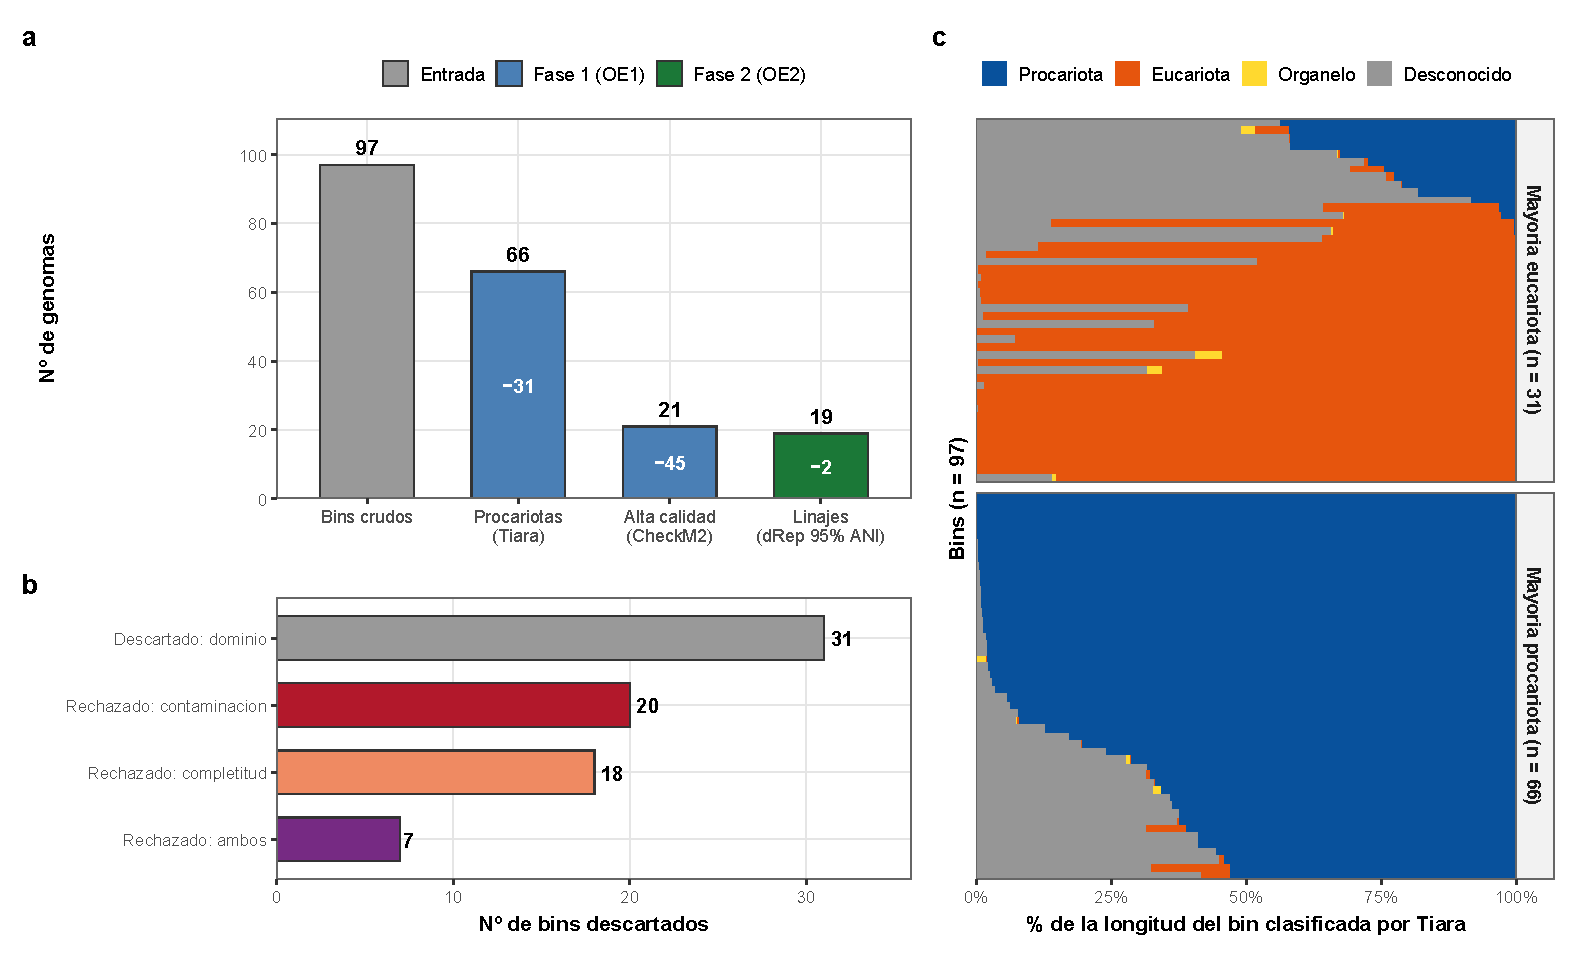
\includegraphics[width=\textwidth]{images/fig1_embudo_seleccion.pdf}
    \caption[Embudo de selección de genomas]{Embudo de selección de genomas
    desde los bins crudos hasta los linajes. \textbf{(a)} Número de genomas que
    sobrevive a cada etapa del flujo: 97 bins crudos procedentes de 22 librerías
    Illumina, 66 con dominio mayoritariamente procariota según Tiara, 21 que
    superan los umbrales de calidad de CheckM2 (completitud superior al
    70\%, contaminación inferior al 5\%) y 19 linajes tras la
    desreplicación con dRep al
    95\% de ANI. Las cifras en blanco indican las pérdidas en cada paso.
    \textbf{(b)} Motivos de descarte de los 76 bins eliminados. \textbf{(c)}
    Composición por dominio de cada uno de los 97 bins según Tiara, expresada
    como porcentaje de la longitud del bin clasificada en cada categoría; los
    bins se separan según su dominio mayoritario y se ordenan por la fracción
    procariota.}
    \label{fig:embudo}
\end{figure}

La Figura~\ref{fig:embudo}(c) muestra que la clasificación por dominio no es
ambigua en la mayoría de los casos: los bins se concentran en los extremos de
la escala, con una fracción procariota cercana al 0\% o al 100\%, y son
pocos los que ocupan posiciones intermedias. Esto respalda la decisión de
aplicar un criterio de mayoría simple sobre la longitud clasificada en lugar de
un umbral más elaborado.

\subsection{Calidad y estructura de los 21 genomas seleccionados}

Los 21 genomas retenidos presentan una calidad marcadamente asimétrica respecto
del umbral. La mediana de la completitud alcanza el 99.86\%, con 13 genomas por
encima del 99\% y 5 con completitud estimada del 100.00\%; solo cuatro
quedan por debajo del 80\%. La mediana de la contaminación es del 0.44\%, valor muy por debajo del límite fijado.

\begin{figure}[H]
    \centering
    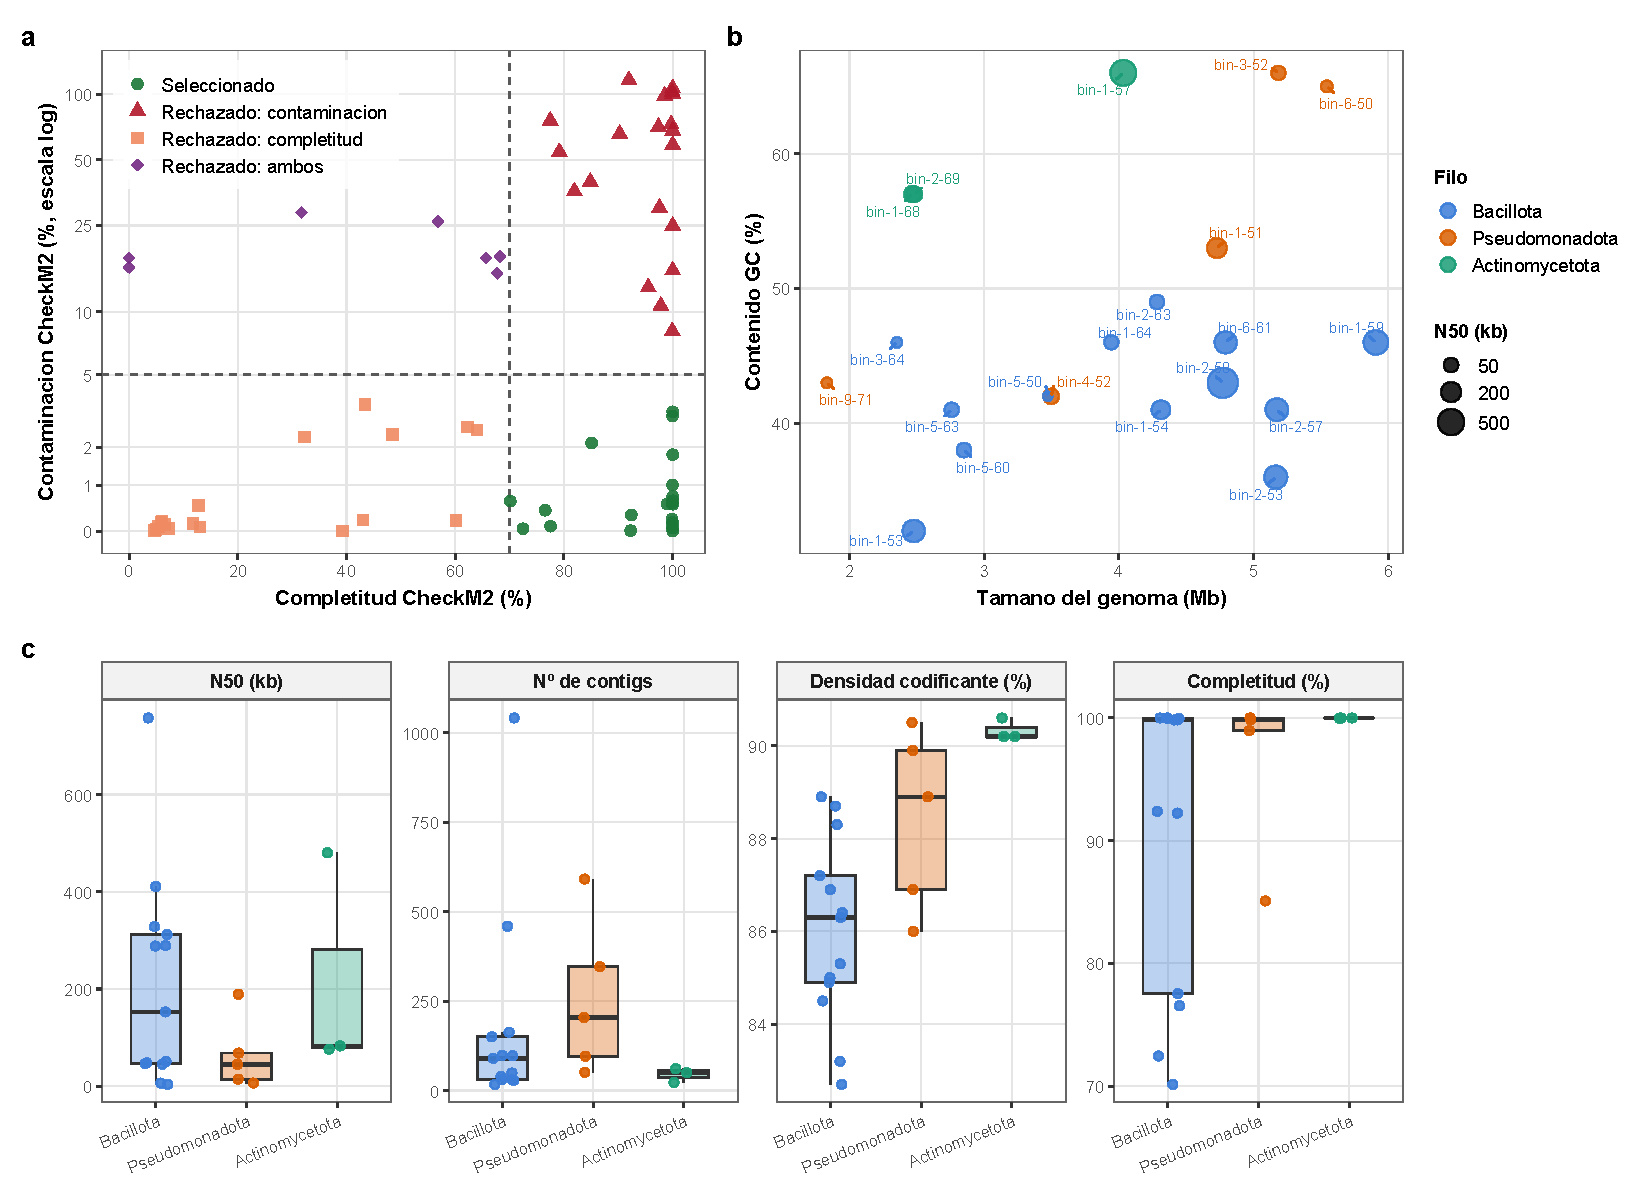
\includegraphics[width=\textwidth]{images/fig2_calidad_genomica.pdf}
    \caption[Calidad y métricas de ensamblaje]{Calidad y métricas de ensamblaje
    de los genomas. \textbf{(a)} Completitud frente a contaminación (CheckM2) de
    los 66 bins procariotas. El eje de contaminación usa escala logarítmica
    ($\log(1+x)$) porque unos pocos bins superan el 60\% y comprimirían la
    región de interés. Las líneas discontinuas marcan los umbrales del estudio
    (completitud igual o superior al 70\%, contaminación inferior al 5\%) y
    la región sombreada, los
    21 genomas seleccionados. \textbf{(b)} Tamaño del genoma frente a contenido
    GC de los 21 genomas seleccionados; el tamaño del punto es proporcional al
    N50 de los contigs y el color indica el filo. \textbf{(c)} Distribución de
    N50, número de contigs, densidad codificante y completitud por filo. Cada
    punto es un genoma; las cajas muestran mediana y cuartiles.}
    \label{fig:calidad}
\end{figure}

La Figura~\ref{fig:calidad}(a) muestra los criterios de contaminación y completitud sobre las distintas poblaciones de bins.

La completitud y la contaminación no describen por completo la utilidad de un
genoma para el análisis pangenómico. La continuidad del ensamblaje sí importa, y
en esa dimensión el conjunto es heterogéneo: el número de contigs va de 17 a
1041, con mediana de 90. Cuatro genomas superan los 300 contigs
(\texttt{bin-5-50} con 1041, \texttt{bin-6-50} con 591, \texttt{bin-3-64} con
459 y \texttt{bin-9-71} con 346).

El caso de \texttt{bin-5-50} muestra que la calidad y la fragmentación de un genoma son aspectos distintos. Este bin tiene una completitud del 76.56\% y una contaminación del 0.44\%, por lo que cumple los criterios del OE1. Sin embargo, sus 3.47 Mb están divididos en más de mil contigs, con una longitud media de solo 3.3 kb.

CheckM2 le asigna una buena calidad porque evalúa principalmente la presencia de genes marcadores, muchos de los cuales pueden encontrarse completos incluso en contigs pequeños. Por tanto, esta métrica no refleja directamente qué tan continuo está el ensamblaje.

El problema aparece en la Fase 3. Cuando un gen queda cortado entre contigs, puede no coincidir correctamente con su versión completa en los genomas de referencia. Como resultado, el análisis pangenómico puede interpretarlo como un gen diferente y clasificarlo como accesorio o incluso exclusivo de la Estela. Así, una alta fragmentación puede generar falsos genes exclusivos, afectando directamente al OE3. Por esta razón, la Fase 3 incluye controles para identificar y descartar estos casos.


Los tamaños genómicos oscilan entre 1.83 y 5.91 Mb, con mediana de 4.03 Mb,
valores compatibles con genomas bacterianos. El extremo inferior
corresponde a \texttt{bin-9-71} (1.83 Mb), cuya completitud del 85.09\%.

\begin{table}[H]
\centering
\small
\caption[Métricas de los 21 MAGs seleccionados]{Métricas de ensamblaje y calidad
genómica de los 21 MAGs seleccionados (completitud superior al 70\% y
contaminación inferior al 5\%).}
\label{tab:bins_seleccionados}
\makebox[\textwidth][c]{%
\begin{tabular}{lrrrrr}
\toprule
\textbf{Bin} & \textbf{Contigs} & \textbf{Longitud (bp)} & \textbf{Dominio} & \textbf{Completitud (\%)} & \textbf{Contaminación (\%)} \\
\midrule
bin-1-51 & 51 & 4.727.435 & prok & 100.00 & 0.00 \\
bin-1-53 & 30 & 2.476.631 & prok & 99.84 & 0.12 \\
bin-1-54 & 49 & 4.312.038 & prok & 92.25 & 0.01 \\
bin-1-57 & 22 & 4.032.412 & prok & 99.99 & 3.23 \\
bin-1-59 & 98 & 5.907.869 & prok & 99.97 & 3.07 \\
bin-1-64 & 163 & 3.944.265 & prok & 99.84 & 0.59 \\
bin-1-68 & 50 & 2.465.224 & prok & 100.00 & 1.79 \\
bin-2-53 & 39 & 5.164.804 & prok & 99.99 & 0.57 \\
bin-2-57 & 28 & 5.172.263 & prok & 99.96 & 1.01 \\
bin-2-58 & 17 & 4.771.531 & prok & 100.00 & 0.06 \\
bin-2-63 & 150 & 4.282.638 & prok & 92.39 & 0.34 \\
bin-2-69 & 61 & 2.481.071 & prok & 99.99 & 0.18 \\
bin-3-52 & 204 & 5.184.467 & prok & 98.97 & 0.58 \\
bin-3-64 & 459 & 2.352.198 & prok & 70.14 & 0.64 \\
bin-4-52 & 96 & 3.497.259 & prok & 99.86 & 0.25 \\
bin-5-50 & 1041 & 3.472.002 & prok & 76.56 & 0.44 \\
bin-5-60 & 97 & 2.849.856 & prok & 77.53 & 0.10 \\
bin-5-63 & 90 & 2.758.939 & prok & 72.46 & 0.05 \\
bin-6-50 & 591 & 5.543.214 & prok & 100.00 & 0.65 \\
bin-6-61 & 30 & 4.792.746 & prok & 100.00 & 0.74 \\
bin-9-71 & 346 & 1.832.072 & prok & 85.09 & 2.13 \\
\bottomrule
\end{tabular}%
}
\end{table}

\subsection{Implicancia para el OE1}

El OE1 se cumple. Obtenemos un conjunto de 21 genomas procariotas cuya
completitud y pureza permiten la asignación taxonómica y la comparación
genómica posteriores. Por ese motivo descartamos 78.35\% del material de
partida. La depuración  descarta
organismos que estuvieran presentes en la estela pero que no alcanzan la calidad necesaria para los posteriores análisis. Por lo tanto, la diversidad
real de la fracción viable es mayor que la que estos 21 genomas representan.

El detalle de todos los 97 bins evaluados, con los motivos específicos para su
exclusión, se presenta en el Anexo~\ref{anexo:tabla_completa_bins}.

\section{Fase 2. Asignación taxonómica y definición de linajes (OE2)}

La Fase 2 se ejecutó en Khipu mediante \texttt{run\_fase2.slurm} (trabajo SLURM
49316) sobre los 21 genomas seleccionados en la fase anterior. El flujo
comprendió la clasificación taxonómica con GTDB-Tk sobre los datos de la versión
R220, la confirmación de especie por ANI, la desreplicación en linajes con dRep
y el cálculo de la prevalencia espacial de cada linaje.

\subsection{Composición taxonómica de la fracción viable}

GTDB-Tk clasificó los 21 genomas dentro de tres filos bacterianos. No se detectó
ningún genoma arqueal, lo que resuelve la ambigüedad que
Tiara había dejado abierta en la Fase 1 entre bacterias y arqueas. La
distribución está dominada por Bacillota, con 13 genomas (62\%), seguido de
Pseudomonadota con 5 (24\%) y Actinomycetota con 3 (14\%). Por debajo del
filo, la diversidad es alta en relación con el tamaño de la muestra: los 21
genomas se reparten en 11 órdenes y 17 géneros distintos, y solo cuatro géneros
aportan más de un genoma.

\begin{figure}[H]
    \centering
    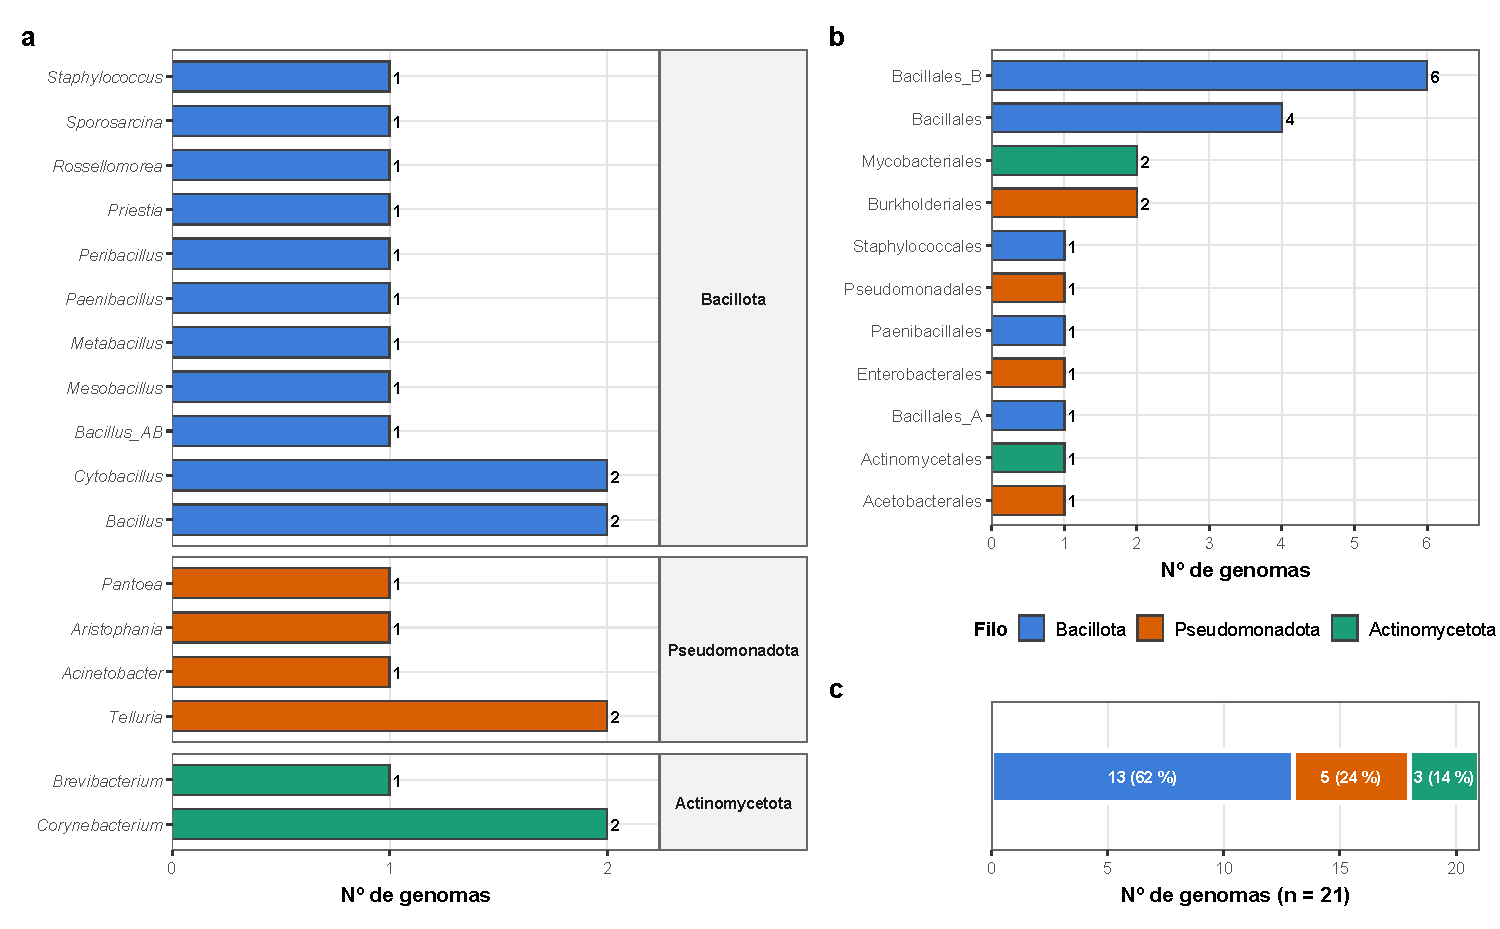
\includegraphics[width=\textwidth]{images/fig7_composicion_taxonomica.pdf}
    \caption[Composición taxonómica]{Composición taxonómica del conjunto de
    genomas seleccionados. \textbf{(a)} Número de genomas por género, agrupados
    por filo. \textbf{(b)} Número de genomas por orden. \textbf{(c)} Reparto de
    los 21 genomas entre los tres filos detectados.}
    \label{fig:composicion}
\end{figure}

El predominio de Bacillota (Figura~\ref{fig:composicion}) es coherente con el
sustrato y con el método de obtención de la muestra. Buena parte de los géneros
recuperados dentro de este filo (\textit{Bacillus}, \textit{Peribacillus},
\textit{Priestia}, \textit{Cytobacillus}, \textit{Metabacillus},
\textit{Rossellomorea}, \textit{Mesobacillus}, \textit{Sporosarcina},
\textit{Paenibacillus}) forma endosporas, una estrategia de resistencia que
favorece la supervivencia sobre una superficie pétrea expuesta a desecación,
radiación ultravioleta y oscilación térmica    \cite{jroundi2020}. 

\subsection{Confirmación filogenómica}

\begin{figure}[H]
    \centering
    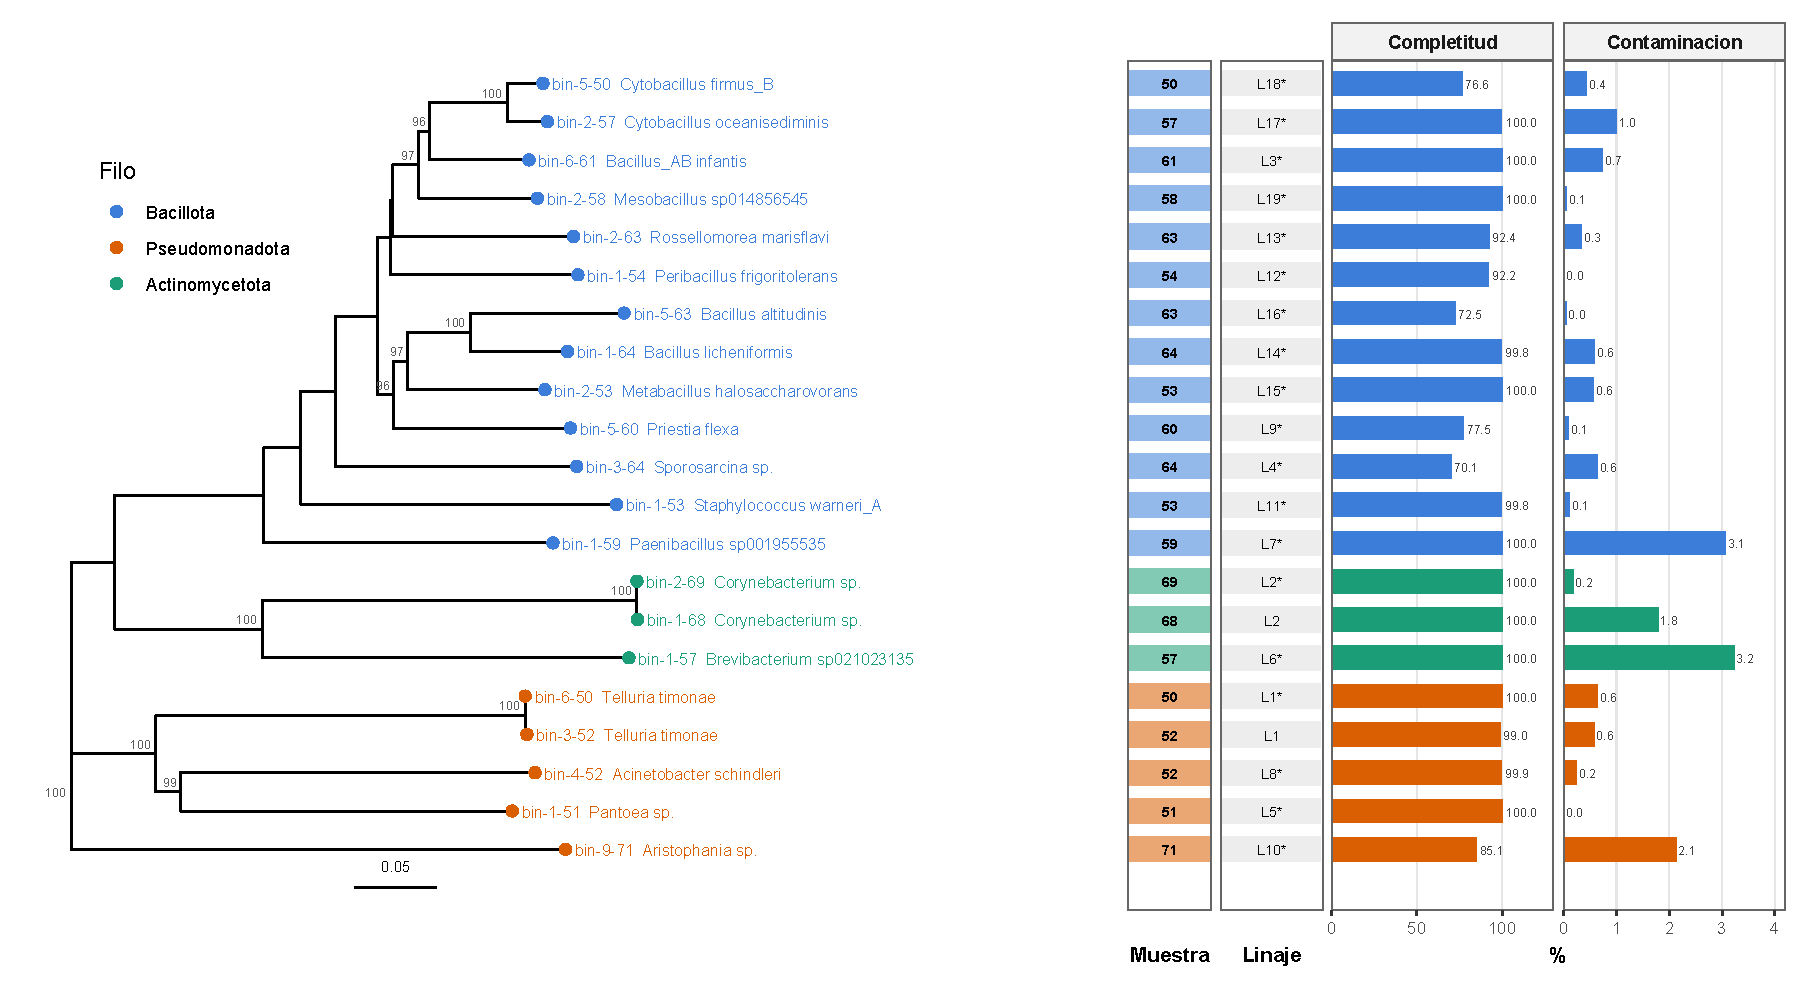
\includegraphics[width=\textwidth]{images/fig3_arbol_filogenomico.pdf}
    \caption[Árbol filogenómico de los 21 genomas]{Árbol filogenómico de los 21
    genomas seleccionados con sus metadatos. Árbol de Neighbor-Joining calculado
    sobre distancias-p a partir del alineamiento concatenado de los 120
    marcadores bacterianos de copia única (bac120, 5035 posiciones) generado por
    GTDB-Tk (datos R220), enraizado en el filo Pseudomonadota. Los números sobre
    las ramas son valores de soporte de \textit{bootstrap} (500 réplicas); solo
    se muestran los iguales o superiores al 70\%. Las columnas de la derecha
    indican, para cada
    genoma, la muestra de origen, el linaje asignado por dRep (el asterisco marca
    el genoma representante del linaje) y los valores de completitud y
    contaminación de CheckM2.}
    \label{fig:arbol}
\end{figure}

La topología del árbol (Figura~\ref{fig:arbol}) es congruente con la asignación
taxonómica: los tres filos se recuperan como grupos separados y los genomas del
mismo género quedan en ramas adyacentes. Los valores de soporte son altos en los
nodos que definen la estructura principal, con \textit{bootstrap} del 100\% en
la separación de los filos y en los pares congenéricos.

El alcance de este resultado es limitado. El árbol es de distancias y se
calculó únicamente sobre los genomas de consulta, sin incorporar genomas de
referencia de GTDB, de modo que verifica la coherencia interna del conjunto pero
no constituye una prueba filogenética independiente de la asignación taxonómica.
Tal como se justificó en el Capítulo IV, el árbol de novo focalizado por linaje,
con referencias del taxón asignado y grupo externo, queda previsto para la
Fase 4.

\subsection{Confirmación de especie y candidatos a novedad taxonómica}

Se calculó la Identidad Nucleotídica Promedio de cada genoma frente a su
referencia GTDB más próxima, aplicando los criterios de confirmación de especie
definidos en el Capítulo IV (ANI $\ge 95\%$ y fracción alineada $\ge 65\%$).
Dieciséis de los 21 genomas satisfacen ambos criterios, con valores de ANI entre
95.61\% y 99.99\% y mediana de 98.53\%. Doce de los 16 superan el 98\% de ANI, lo que indica correspondencias con especies
descritas.

\begin{figure}[H]
    \centering
    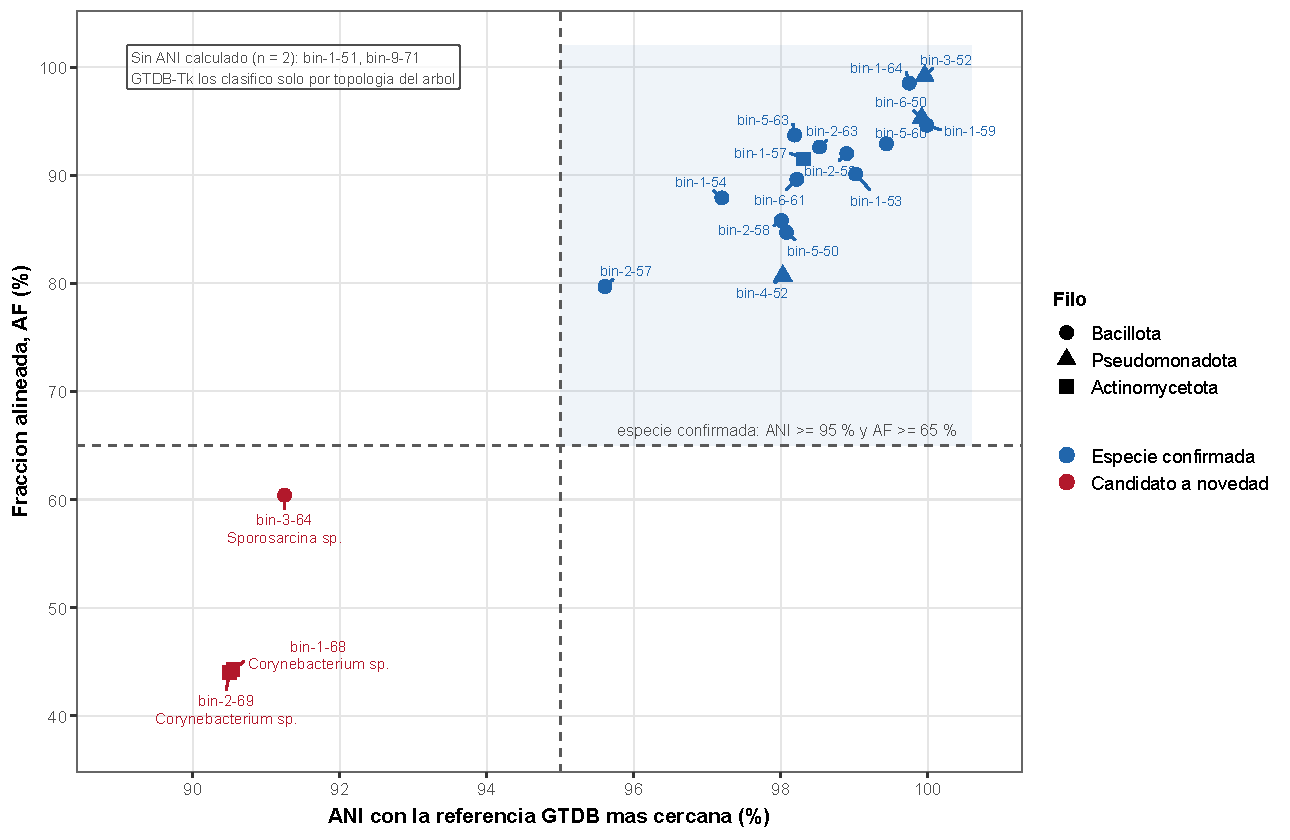
\includegraphics[width=0.85\textwidth]{images/fig5_novedad_taxonomica.pdf}
    \caption[Evaluación de novedad taxonómica]{Evaluación de novedad taxonómica
    frente a la referencia GTDB más cercana. ANI frente a fracción alineada (AF)
    de cada genoma respecto de su referencia GTDB más cercana. Las líneas
    discontinuas marcan los criterios de confirmación de especie (ANI
    igual o superior al 95\% y AF igual o superior al 65\%). Los 16 genomas
    del cuadrante sombreado
    tienen especie confirmada. Dos genomas adicionales (\texttt{bin-1-51},
    \textit{Pantoea} sp., y \texttt{bin-9-71}, \textit{Aristophania} sp.) fueron
    clasificados únicamente por topología del árbol, sin cálculo de ANI, y no
    aparecen representados.}
    \label{fig:novedad}
\end{figure}

Los 5 genomas restantes se distribuyen en dos situaciones distintas
(Figura~\ref{fig:novedad}). Dos de ellos, \texttt{bin-1-51}
(\textit{Pantoea} sp.) y \texttt{bin-9-71} (\textit{Aristophania} sp.), fueron
ubicados por GTDB-Tk mediante la topología del árbol de colocación sin que se
calculara ANI, de modo que su clasificación se detiene en el rango de género por
ausencia de una referencia suficientemente próxima. Por ese motivo, esas secuencias se descartan para la fase 3.

Los otros 3 sí produjeron valores de ANI, pero por debajo del umbral de
especie, y constituyen el hallazgo taxonómico más relevante de esta fase. Los
dos genomas de \textit{Corynebacterium} sp. (\texttt{bin-1-68} y
\texttt{bin-2-69}) alcanzan un ANI de 90.55 y 90.50\% frente a su referencia
más cercana, con fracciones alineadas de apenas 44,3 y 44.0\%. El genoma de
\textit{Sporosarcina} sp. (\texttt{bin-3-64}) queda en 91.25\% de ANI y
60.4\% de AF. Los tres valores de ANI se encuentran por debajo del umbral de similitud utilizado para la circunscripción de especies en GTDB, lo que indica que ninguno de estos genomas puede asignarse a la misma especie que su referencia más cercana. 

En el caso de los \textit{Corynebacterium}
la fracción alineada, inferior al 45\%, indica que menos de la mitad del genoma
encuentra correspondencia en la referencia. Estos genomas son, por tanto,
candidatos a especies no descritas en la versión R220 del GTDB. 

Hacemos énfasis en este resultado porque ambos \textit{Corynebacterium} proceden de muestras
distintas y presentan completitud del 100\%, de modo que la divergencia
observada no es atribuible a una reconstrucción defectuosa.

\subsection{Desreplicación y definición de linajes}

La desreplicación con dRep agrupó los 21 genomas en 19 linajes, definidos como
clústeres de especie al 95\% de ANI. Solo dos pares colapsaron.

\begin{figure}[H]
    \centering
    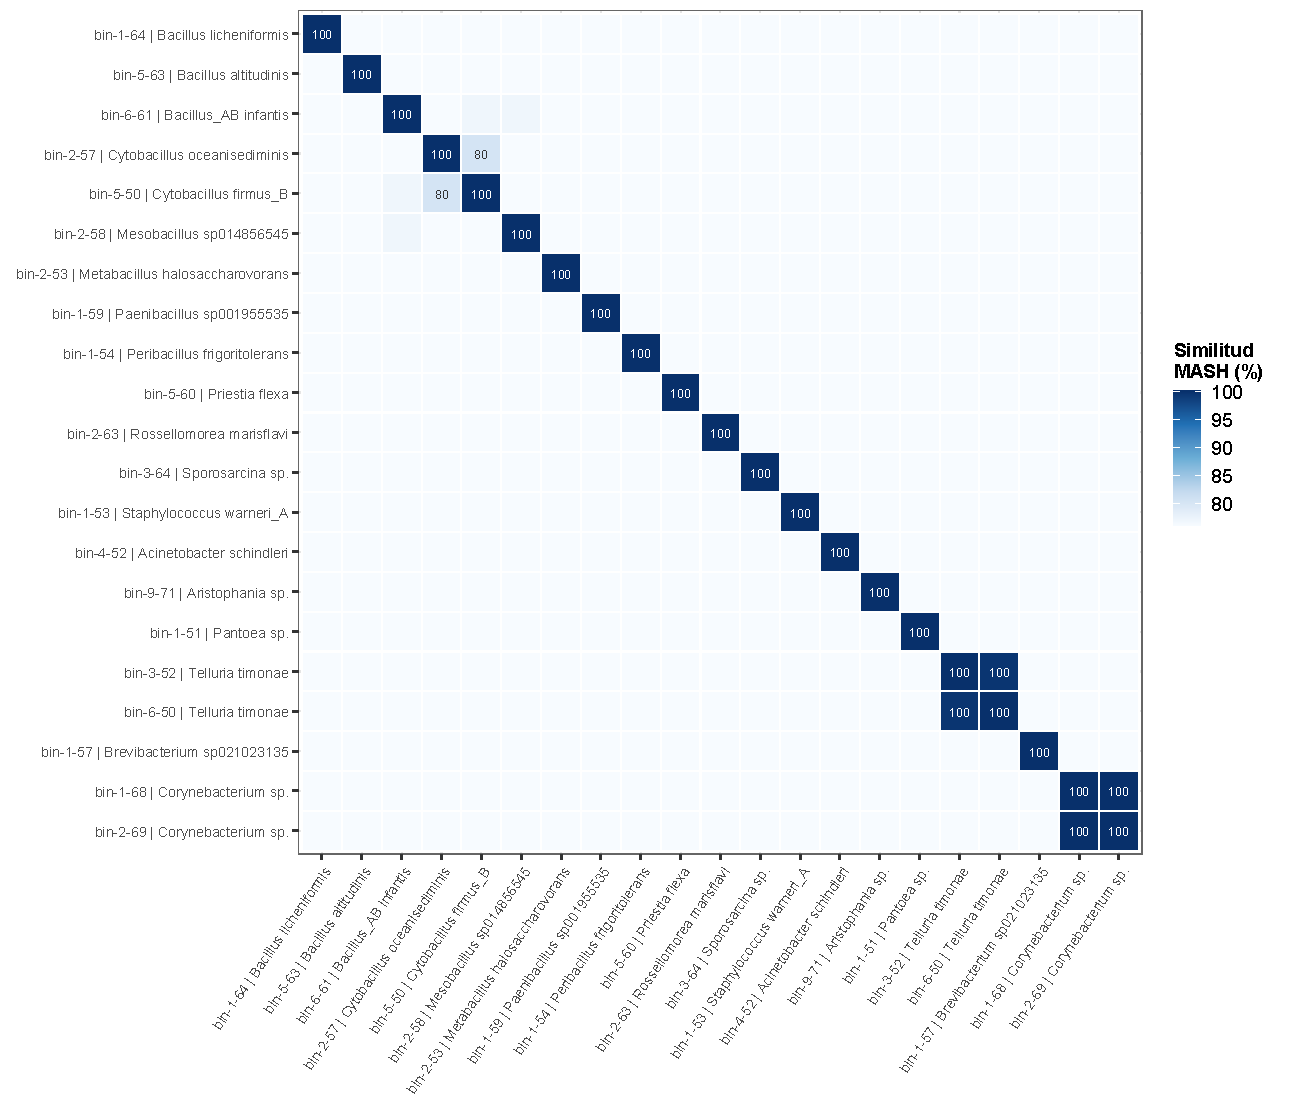
\includegraphics[width=0.9\textwidth]{images/fig4_matriz_mash.pdf}
    \caption[Matriz de similitud genómica]{Matriz de similitud genómica entre
    los 21 genomas seleccionados. Similitud MASH ($100 -$ distancia MASH) entre
    todas las parejas de genomas, ordenadas por filo y género. Solo dos parejas
    presentan similitud máxima: los dos \textit{Telluria timonae} (muestras 50 y
    52) y los dos \textit{Corynebacterium} sp. (muestras 68 y 69). Nota
    metodológica: dRep ejecuta fastANI únicamente dentro de cada clúster primario
    definido por MASH, de modo que no existe una matriz de ANI completa para los
    21 genomas; la matriz de todos contra todos disponible es la de MASH.}
    \label{fig:mash}
\end{figure}

Las dos parejas sometidas a fastANI dentro de su clúster primario superan el
umbral de especie con amplitud: \textit{Corynebacterium} sp.
(\texttt{bin-1-68} $\leftrightarrow$ \texttt{bin-2-69}) alcanza 99.96\% de ANI
con 97.1\% de cobertura del alineamiento, y \textit{Telluria timonae}
(\texttt{bin-3-52} $\leftrightarrow$ \texttt{bin-6-50}), 99.78\% de ANI con
85.2\% de cobertura. Ambas colapsan en un único linaje.

El resto de los genomas resulta mutuamente distante
(Figura~\ref{fig:mash}), incluido el par de \textit{Cytobacillus}
(\texttt{bin-5-50} y \texttt{bin-2-57}), que pese a compartir género se mantiene
como dos linajes separados con una similitud MASH del 80\%. Este es el motivo
de que 21 genomas den lugar a 19 linajes y no a un número menor: la redundancia
entre muestras es baja, y la mayor parte de lo recuperado corresponde a
organismos distintos y no a reconstrucciones repetidas del mismo genoma.

\subsection{Prevalencia espacial de los linajes}

\begin{figure}[H]
    \centering
    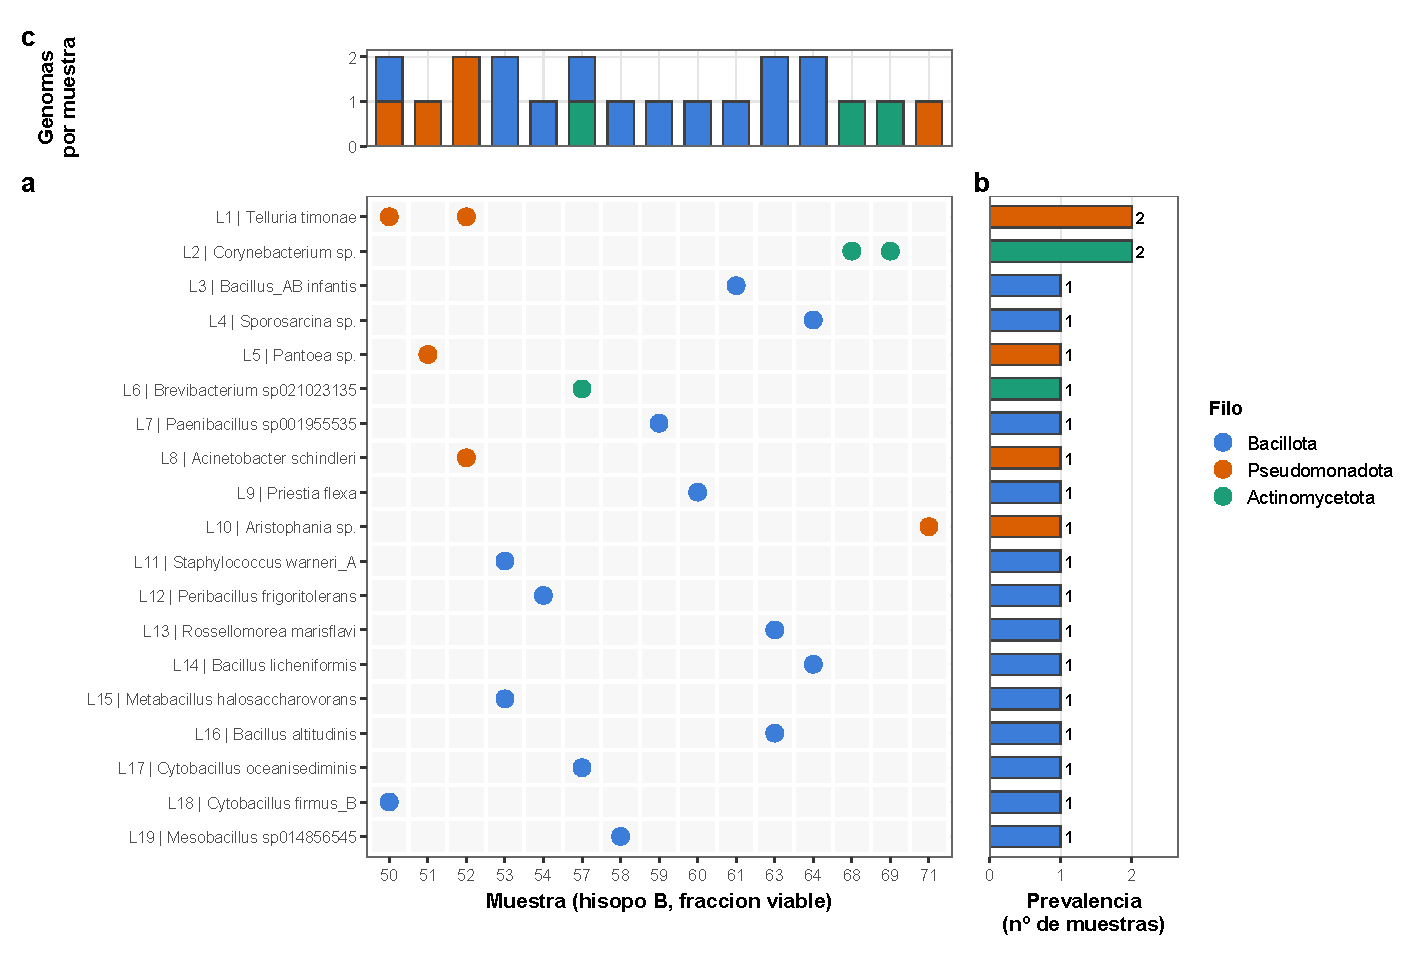
\includegraphics[width=\textwidth]{images/fig6_prevalencia_linajes.pdf}
    \caption[Prevalencia espacial de los linajes]{Prevalencia espacial de los
    linajes. \textbf{(a)} Matriz de presencia de cada linaje (filas, ordenadas
    por prevalencia descendente) en cada muestra (columnas); el color indica el
    filo. \textbf{(b)} Prevalencia de cada linaje, definida como el número de
    muestras distintas en que aparece, coloreada por filo. \textbf{(c)} Número de
    genomas de alta calidad recuperados por muestra, coloreado por filo.
    Limitación: la prevalencia se calcula sobre el número de muestras y no sobre
    zonas físicas de la estela, porque no se dispone de un mapeo
    muestra $\rightarrow$ zona en formato analizable.}
    \label{fig:prevalencia}
\end{figure}

La prevalencia espacial resultó baja en todo el conjunto. Diecisiete de los 19
linajes aparecen en una sola muestra, y solo dos alcanzan una prevalencia de
dos: L1 (\textit{Telluria timonae}, muestras 50 y 52) y L2
(\textit{Corynebacterium} sp., muestras 68 y 69). Ningún linaje se recuperó en
tres o más puntos. Además, de las 22 librerías que produjeron bins, solo 15
aportaron al menos un genoma de alta calidad tras la Fase 1
(Figura~\ref{fig:prevalencia}(c)).

Este resultado limita el poder discriminante de la métrica. Con un rango
efectivo de apenas dos valores, la prevalencia no permite ordenar los linajes ni separar con seguridad a los colonizadores
estables de las detecciones puntuales.

Dos hipotésis resultan compatibles con los datos. La primera es que la comunidad
viable de la estela sea genuinamente heterogénea entre muestras, sin un núcleo de
organismos compartido. La segunda es que la recuperación de genomas de alta calidad sea limitada, de modo que un linaje presente en varias muestras solo pueda reconstruirse con suficiente calidad en una de ellas.

Los datos disponibles no permiten discriminar entre ambas. La segunda tampoco puede descartarse, dado que el flujo retuvo apenas el 21.65\% de los bins iniciales.

Por esta razón, la prevalencia espacial se reporta aquí como caracterización de
la distribución de cada linaje sobre el monumento, pero no se emplea como
criterio para decidir qué especies ingresan al análisis pangenómico. 

Por ese motivo, el criterio de selección de bins para el pangenoma (fase 3) cambia como se explica en la siguiente sección. 

\subsection{Implicancia para el OE2}

El OE2 se cumple: los 21 genomas quedan clasificados con resolución de especie
en 16 casos y de género en los 5 restantes, y agrupados en 19 linajes
operativos que constituyen la unidad de análisis de las fases siguientes.

Dos resultados condicionan el diseño posterior. El primero es la baja
redundancia entre muestras: con 19 linajes sobre 21 genomas, y 17 de ellos
representados por un único genoma, no es posible construir un pangenoma
empleando exclusivamente material de la estela. El análisis pangenómico de la
Fase 3 debe apoyarse necesariamente en conjuntos de genomas de referencia
públicos. El segundo es la detección de tres candidatos a especies no descritas,
entre ellos los dos \textit{Corynebacterium} de completitud íntegra, que por
carecer de referencia comparable quedan fuera del análisis pangenómico pero
constituyen un hallazgo reportable por sí mismo.

\begin{table}[H]
\centering
\footnotesize
\setlength{\tabcolsep}{4pt}
\caption[Linajes definidos en la Fase 2]{Linajes definidos en la Fase 2,
ordenados por prevalencia espacial descendente.}
\label{tab:linajes}
\makebox[\textwidth][c]{%
\begin{tabular}{llrlll}
\toprule
\textbf{Linaje} & \textbf{Taxonomía (GTDB)} & \textbf{Prev.} & \textbf{Muestras} & \textbf{Representante} & \textbf{Especie conf.} \\
\midrule
L1  & \textit{Telluria timonae}              & 2 & 50, 52 & bin-6-50 & Sí \\
L2  & \textit{Corynebacterium} sp.           & 2 & 68, 69 & bin-2-69 & No \\
L3  & \textit{Bacillus\_AB infantis}         & 1 & 61 & bin-6-61 & Sí \\
L4  & \textit{Sporosarcina} sp.              & 1 & 64 & bin-3-64 & No \\
L5  & \textit{Pantoea} sp.                   & 1 & 51 & bin-1-51 & --- \\
L6  & \textit{Brevibacterium} sp021023135    & 1 & 57 & bin-1-57 & Sí \\
L7  & \textit{Paenibacillus} sp001955535     & 1 & 59 & bin-1-59 & Sí \\
L8  & \textit{Acinetobacter schindleri}      & 1 & 52 & bin-4-52 & Sí \\
L9  & \textit{Priestia flexa}                & 1 & 60 & bin-5-60 & Sí \\
L10 & \textit{Aristophania} sp.              & 1 & 71 & bin-9-71 & --- \\
L11 & \textit{Staphylococcus warneri\_A}     & 1 & 53 & bin-1-53 & Sí \\
L12 & \textit{Peribacillus frigoritolerans}  & 1 & 54 & bin-1-54 & Sí \\
L13 & \textit{Rossellomorea marisflavi}      & 1 & 63 & bin-2-63 & Sí \\
L14 & \textit{Bacillus licheniformis}        & 1 & 64 & bin-1-64 & Sí \\
L15 & \textit{Metabacillus halosaccharovorans} & 1 & 53 & bin-2-53 & Sí \\
L16 & \textit{Bacillus altitudinis}          & 1 & 63 & bin-5-63 & Sí \\
L17 & \textit{Cytobacillus oceanisediminis}  & 1 & 57 & bin-2-57 & Sí \\
L18 & \textit{Cytobacillus firmus\_B}        & 1 & 50 & bin-5-50 & Sí \\
L19 & \textit{Mesobacillus} sp014856545      & 1 & 58 & bin-2-58 & Sí \\
\bottomrule
\end{tabular}%
}

\vspace{0.5em}
\begin{minipage}{0.95\textwidth}
\footnotesize
\textit{Nota.} Prev.: prevalencia espacial, número de muestras distintas que
aportan al menos un genoma al linaje. Especie conf.: confirmación de especie por
ANI igual o superior al 95\% y AF igual o superior al 65\%; el guion indica
los linajes clasificados por
topología del árbol, sin cálculo de ANI. Los sufijos \texttt{\_A} y \texttt{\_B}
y los epítetos alfanuméricos del tipo \texttt{sp}$\langle$dígitos$\rangle$
corresponden a la nomenclatura propia del GTDB.
\end{minipage}
\end{table}
